\documentclass{article}
\title{CSC355 PS3}
\author{Alex Zhang}
\date{March 2024}
\textwidth=16.00cm 
\textheight=22.00cm 
\topmargin=0.00cm
\oddsidemargin=0.00cm 
\evensidemargin=0.00cm 
\headheight=0cm 
\headsep=0.5cm
\textheight=610pt
\usepackage{graphicx}
\usepackage{multicol}


\graphicspath{ {./images/} }

\usepackage{latexsym,array,delarray,amsthm,amssymb,epsfig}
\usepackage{amsmath}
\usepackage{listings}
\lstset{
  basicstyle=\ttfamily,
  mathescape
}

\newcommand{\bmat}[1]{\begin{bmatrix} #1 \end{bmatrix}}
\newcommand{\mat}[1]{\mathbf{#1}}

\let\ds\displaystyle

\begin{document}
\maketitle
\section*{Problem 1}
Let $g(x) = \sum^n_{k=0}L_k(x)$. 
If we plug in all points from $x_0,\dots,x_n$ into $g(x)$, we will get $g(x_k) = 1, \forall k = 0,\dots,n$.
Because $L_k(x_k)$, as a lagrange basis, will be 1 and be 0 for other $k$.
We also know that because each $L_k(x)$ is a n-degree polynomial, their summation will be a polynomial with at most n degree, which is $g(x)$.
\\
Instead of representing $g(x)$ in lagrange basis, we can try to represent $g(x)$ into monomial basis which is 
$$g(x) = a_0 + a_1x + a_2x^2 + \dots + a_nx^n$$
We also have total n+1 function values at $g(x_k)$ for $k=0,\dots,n$. And we can create its Vandermonde matrix and a linear system.
$$\bmat{1 & x_0 & \cdots & x_0^n\\
        1 & x_1 & \cdots & x_1^n\\
        \vdots & \vdots & \ddots & \vdots\\
        1 & x_n & \cdots & x_n^n\\} \cdot \bmat{a_0 \\a_1 \\ \vdots \\a_n} = \bmat{1\\1\\\vdots\\1}$$
Since this Vandermonde matrix is a square matrix, it has an unique solution.
Through observation, we can see the solution is when $a_0 = 1$, and everything else to be $0$. This means our $g(x) = 1$.
So $\sum^n_{k=0}L_k(x) = 1.\blacksquare$





\section*{Problem 2}
\subsection*{(a)}
Coefficients for Newton basis with the given point are,
$$\bmat{0.0379    &   0.0856  &     0.1632 &     0.34133 &    0.029562 &     -1.0447     &  1.9711  &    -2.5477  &     2.5997}$$
\subsection*{(b)}
The evaluation values at these points are,
$$\bmat{0.043428   &   0.35741  &    0.47629    &      0.5   &   0.46928  &    0.34266  &   0.039373}$$
\subsection*{(c)}
The function values using polyfit and polyval is,
$$\bmat{0.043428    &  0.35741 &     0.47629    &      0.5 &     0.46928  &    0.34266   &  0.039373}$$
The relative error between function value from polyval and my newton's evaluation method is around $1e-14$ for $x= \pm1$.
The error becomes smaller to $1e-16$ as we approaching to the middle point.


\section*{Problem 3}
Based on the problem, we will have three cubic spline polynomials.
\begin{align}
    S_0(x) &= a_0 + b_0(x-x_0) + c_0(x-x_0)^2 + d_0(x-x_0)^3 \nonumber \\
    S_1(x) &= a_1 + b_1(x-x_1) + c_1(x-x_1)^2 + d_1(x-x_1)^3 \nonumber \\
    S_2(x) &= a_2 + b_2(x-x_2) + c_2(x-x_2)^2 + d_2(x-x_2)^3 \nonumber
\end{align}
There will be 12 equations for constraints and they are,
\begin{align}{}
    S_0(x_0) &= f(x_0) \\
    S_0(x_1) &= f(x_1)  \\ 
    S_1(x_1) &= f(x_1) \\
    S_1(x_2) &= f(x_2)  \\
    S_2(x_2) &= f(x_2) \\
    S_2(x_3) &= f(x_3) \\
    S_0^\prime(x_1) &= S_1^\prime(x_1) \\
    S_1^\prime(x_2) &= S_2^\prime(x_2) \\
    S_0^{\prime\prime}(x_1) &= S_1^{\prime\prime}(x_1) \\
    S_1^{\prime\prime}(x_2) &= S_2^{\prime\prime}(x_2) \\
    S_0^{\prime\prime}(x_0) &= 0\\
    S_2^{\prime\prime}(x_3) &= 0
\end{align}
Substitute all with $x_1 = x_0 + h$, $x_2 = x_0+ 2h$, $x_3 = x_0 + 3h$, and cubic polynomials.
\setcounter{equation}{0}
\begin{align}
    a_0 &= f(x_0) \\
    a_0 + b_0h + c_0h^2 + d_0h^3 &= f(x_1) \\
    a_1 &= f(x_1)\\
    a_1 + b_1h + c_1h^2 + d_1h^3 &= f(x_2) \\
    a_2 &= f(x_2)\\
    a_2 + b_2h + c_2h^2 + d_2h^3 &= f(x_3) \\
    b_0 + 2c_0h + 3d_0h^2 &= b_1 \\
    b_1 + 2c_1h + 3d_1h^2 &= b_2 \\
    2c_0 + 6d_0h &= 2c_1\\
    2c_1 + 6d_1h &= 2c_2\\
    2c_0 &= 0\\
    2c_2 + 6d_2h &= 0
\end{align}
With simplification,
\setcounter{equation}{0}
\begin{align}
    a_0 &= f(x_0)\nonumber\\
    a_1 &= f(x_1)\nonumber\\
    a_2 &= f(x_2)\nonumber\\
    b_1 &= b_0 + 3d_0h^3 \\
    b_2 &= b_1 + 6d_0h^3 + 3d_1h^3\\
    c_0 &= 0\nonumber\\
    c_1 &= 3d_0h \nonumber\\
    c_2 &= 3d_0h + 3d_1h \nonumber\\
    d_0h + d_1h + d_2h &= 0 \\
    b_0h + d_0h^3 &= f(x_1) - f(x_0)\\
    b_1h + 3d_0h^3 + d_1h^3 &= f(x_2) - f(x_1)\\
    b_2h + 3d_0h^3 + 3d_1h^3 + d_2h^3 &= f(x_3) - f(x_2)
\end{align}

The 12 equations above will become the linear system for this cubic spline





\section*{Problem 4}
\subsection*{MATLAB's Spline Approximation}
The result plot from $-1$ to $1$ is,
\begin{center}
    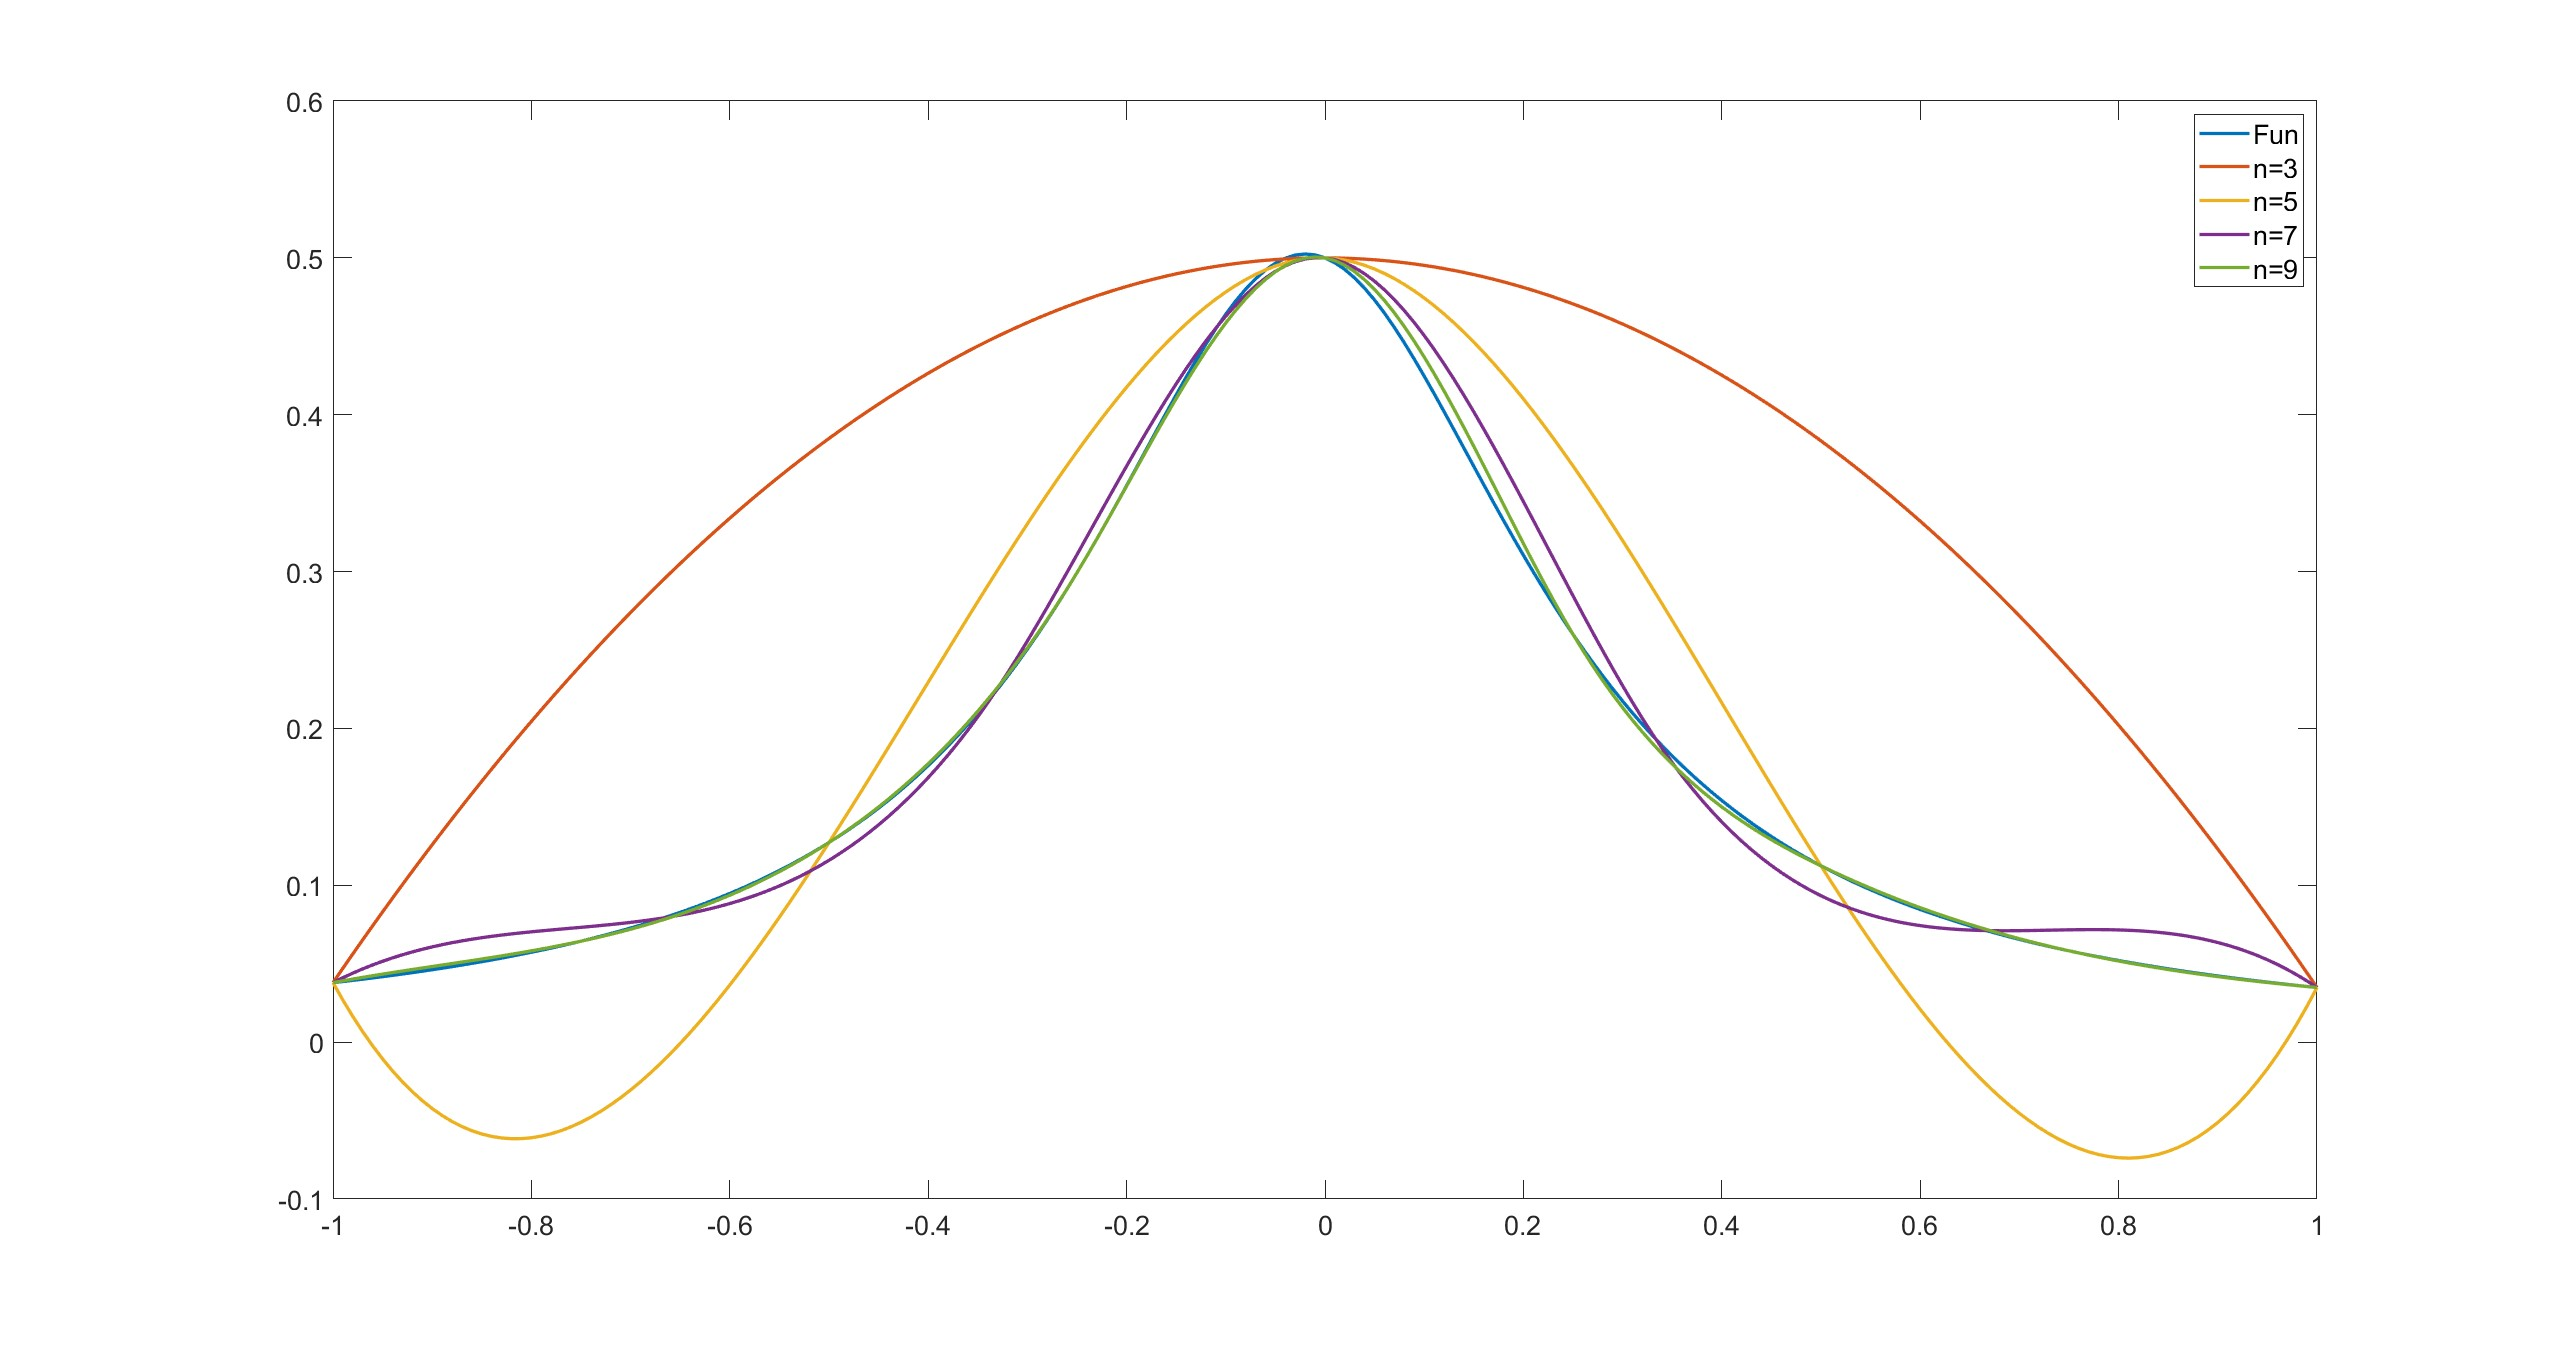
\includegraphics[scale = 0.2]{ps3_q41.jpg}
\end{center}
The coefficients of the polynomial for n=7 is, (left most is the coefficient for $(x-x_i)^3$)
$$\bmat{1.5973   &   -1.1383    &  0.32581  &   0.037925\\
1.5973     & 0.45903  &   0.099386 &    0.079211\\
-7.1174    &   2.0564  &    0.93785      & 0.2225\\
7.4753     &  -5.061   & -0.063694       &   0.5\\
-2.0279    &   2.4143   &  -0.94594     &  0.1933\\
-2.0279    &  0.38636   &  -0.01239    &  0.07113}$$











\subsection*{Single Polynomial}
the coefficients of polynomial of all cases are, (left most is the highest degree).
\\
For 7 points,
$$\bmat{-4.6497  & -0.1183 &   7.6023 &   0.1790  & -3.4162 &  -0.0622 &   0.5000}$$
For 9 points,
$$\bmat{15.4153  &  0.6104&  -30.1368 &  -1.1445 &  18.8478  &  0.6474 &  -4.5900  & -0.1148  &  0.5000}$$
For 11 points,
$$\bmat{-50.8766  & -2.7658 & 116.0274 &   6.1430 & -92.6163  & -4.6473  & 32.3396  &  1.4295  & -5.3378  & -0.1610\\ 0.5000}$$
For 13 points,
$$\bmat{167.1157 &  11.6309 &-435.9938 & -29.7878 & 422.5907  & 27.9182 &-193.5345 & -11.9514  & 45.1281  &  2.3835  \\ -5.7699  & -0.1951   & 0.5000}$$
For 15 points,
$$\bmat{-546.6420 & -46.6521&  1606.5310&   135.2212&    -1830.1796&   -150.5143&    1039.7656&     82.0073&    -319.4911&  -23.1852\\ 55.5576&   3.3391&  -6.0050& -0.2176&   0.5000}$$
\subsection*{Cubic Spline}
The coefficients for different polynomials are represented in matrix form, which each row means coefficients for a certain interval. 
They all follows $f(x) = a(x-x_i)^3 + b(x-x_i)^2 + c(x-x_i) + d$ expression.
\\
For 7 points,
$$\bmat{1.5973    &  -1.1383  &    0.32581  &   0.037925\\
1.5973    &  0.45903   &  0.099386   &  0.079211\\
-7.1174    &   2.0564   &   0.93785   &    0.2225\\
7.4753     &  -5.061  &  -0.063694     &     0.5\\
-2.0279    &   2.4143   &  -0.94594     &  0.1933\\
-2.0279     & 0.38636  &   -0.01239     & 0.07113}$$
For 9 points,
$$\bmat{0.68011   &  -0.21836 &     0.11787   &  0.037925\\
0.68011   &   0.29172    &  0.13621   &  0.064371\\
 1.2475    &   0.8018    &  0.40959   &   0.12728\\
-10.814    &   1.7374    &   1.0444   &   0.29928\\
 11.964    &  -6.3732   &  -0.11456    &      0.5\\
-2.9205    &      2.6   &   -1.0579    &  0.25997\\
-0.21786   &   0.40963  &   -0.30546   &   0.11238\\
-0.21786   &   0.24623  &   -0.14149   &  0.058209}$$
For 11 points,
$$\bmat{ 0.26668  &   0.066301  &   0.072992  &   0.037925\\
0.26668   &   0.22631  &    0.13151  &   0.057309\\
 1.9124   &   0.38632  &    0.25404  &   0.094797\\
-1.3183   &    1.5337  &    0.63805  &    0.17636\\
-12.894   &   0.74274  &     1.0933  &    0.35477\\
 15.189   &   -6.9934  &   -0.15678  &        0.5\\
-1.8644   &    2.1203  &    -1.1314  &    0.31042\\
-1.0143   &    1.0016  &   -0.50702  &    0.15404\\
-0.33462  &    0.39302 &    -0.22809 &    0.084587\\
-0.33462  &    0.19225 &    -0.11103 &    0.052014}$$
For 13 points,
$$\bmat{0.36753  &   0.009349  &   0.079905  &   0.037925\\
0.36753   &   0.19311   &   0.11365   &  0.053204\\
0.61092   &   0.37688   &   0.20865   &  0.079211\\
 2.6071   &   0.68234   &   0.38518   &   0.12728\\
-4.8436   &    1.9859   &   0.82989   &    0.2225\\
-13.568   &  -0.43592   &    1.0882   &   0.39356\\
 17.191   &   -7.2202   &   -0.1878   &       0.5\\
0.21864   &    1.3755   &   -1.1619   &   0.34773\\
-1.7209   &    1.4848   &  -0.68519   &    0.1933\\
-0.64355  &    0.62437  &   -0.33366  &    0.11238\\
-0.27561  &     0.3026  &   -0.17917  &    0.07113\\
-0.27561  &    0.16479  &   -0.10127  &   0.048398}$$
For 15 points,
$$\bmat{0.26209   &  0.060999  &   0.074146  &   0.037925\\
0.26209   &   0.17332   &   0.10762  &   0.050526\\
0.69417   &   0.28565   &   0.17319  &   0.070202\\
 1.0302   &   0.58315   &    0.2973  &     0.1028\\
 2.5123   &    1.0247   &   0.52699  &    0.16017\\
-8.5664   &    2.1014   &   0.97357  &    0.26369\\
 -13.23   &     -1.57   &    1.0495  &    0.42068\\
 18.187   &   -7.2398   &  -0.20905  &        0.5\\
 2.8546   &   0.55463   &   -1.1641  &    0.37541\\
-2.0699   &     1.778   &  -0.83084  &    0.22875\\
-0.96593  &    0.89094  &   -0.44956 &     0.14031\\
-0.54388  &    0.47697  &   -0.25414 &    0.091457\\
-0.22287  &    0.24388  &   -0.15116 &      0.0633\\
-0.22287  &    0.14837  &  -0.095128 &    0.046033}$$
\\
The 10 approximations to the integral are,
\begin{verbatim}
    >> integral_approx
Single interpolating polynomial:
-------------------------------------
Points       Integral value
    7             0.434959
    9             0.294270
   11             0.449111
   13             0.256646
   15             0.508593

Piecewise cubic polynomial:
-------------------------------------
Points       Integral value
    7             0.374510
    9             0.365390
   11             0.364625
   13             0.364522
   15             0.364483
\end{verbatim}
I wil trust the last value from cubic spline. Because I used MATLAB integral function to also compute function's integral.
It seems that 0.36448 is really close to the value I got from MATLAB integral.
\\
I believe about 4 decimal digits are correct. First is I try to test my integral value with more points.
It seems that the value will converge to 0.364471, so the first 4 digits are correct.
\\
Second idea is I tried to represent each cubic spline polynomials into lagrange basis.
Then I can get an error for each cubic polynomial which is $\frac{f^{(4)}(c(x))}{24}(x-x_i)^4$.
Because we are taking the integral, the error should be bounded by 
$$\frac{\max{f^{(4)}(c(x))}}{24\cdot5}(x-x_i)^5 |^{x_{i+1}}_{x_i}$$
Because the lower bound is $x_i$, the evaluation will be 0, which means our integral value will be 
$$\frac{\max{f^{(4)}(c(x))}}{120}h^5$$
where $h$ is the space between each point(we have equispaced points so $h$ will be the same).
Evaluating fourth derivative through MATLAB syms, we get the final error to be $0.00098172$.
I guess this suggest we should be confident with 3 decimal points but consider this is an approximation, 4 decimal digits may work.




\end{document}